\section{Hot Swap Prototype}

	As briefly mentioned above, a protoype was constructed during the fall semester to verify the hot swapping design.  See Figure \ref{fig:prototype} for images of this device.  Measurements taken on this prototype indicated that the signal quality and functional improvements were on track.  Several issues noticed that were corrected in the final design included

	\begin{itemize}
		\item Changing the multiple-height mate-last break-first pogo pin design to a same-height one because of contact issues with the plate electrodes.
		\item Power supply noise from the external switching regulator were undesireable (located at 20kHz on the upper edge of the audible spectrum), so a common mode choke was added in series with the input 24VDC supply to reduce this issue, which was verified experimentally.  The common mode choke functions like a pair of series inductors on both the power and ground lines to reduce high frequency noise that was present on the power supply.
	\end{itemize}

	\begin{sidewaysfigure}
		\centering
		\begin{subfigure}{0.45\textwidth}
			\includegraphics[width = \textwidth]{FinalImages/PrototypeIm.jpg}
			\caption{Prototype device designed, built, and tested in the fall semester.  It contained a single hot swapping receiver.}
		\end{subfigure}
		\begin{subfigure}{0.45\textwidth}
			\includegraphics[width = \textwidth]{FinalImages/PrototypewPedal.jpg}
			\caption{The same prototype with a plate and attached pedal inserted into the hot swapping receiver.}
			\label{fig:NF_AP_sum}
		\end{subfigure}
		\caption{Hot swapping device prototype.}
		\label{fig:prototype}
	\end{sidewaysfigure}

\section{Module Circuit Board Layouts}

	\subsection{Circuit Board Hierarchy}

	For maximum flexibility in mechanical design, each module uses a hierarchical design, in addition to its inherent modularity with respect to the complete device.  All of the computation and routing controls for a module is located on a main circuit board. This main board is connected to the two sets of pogo pins discussed in the receiver design section. It is also connected to the circuit boards that contain the switches for the user interface. A block diagram of this connection system is shown in Figure \ref{fig:ModulePCBHierarchy}.

	\begin{figure}
		\centering
		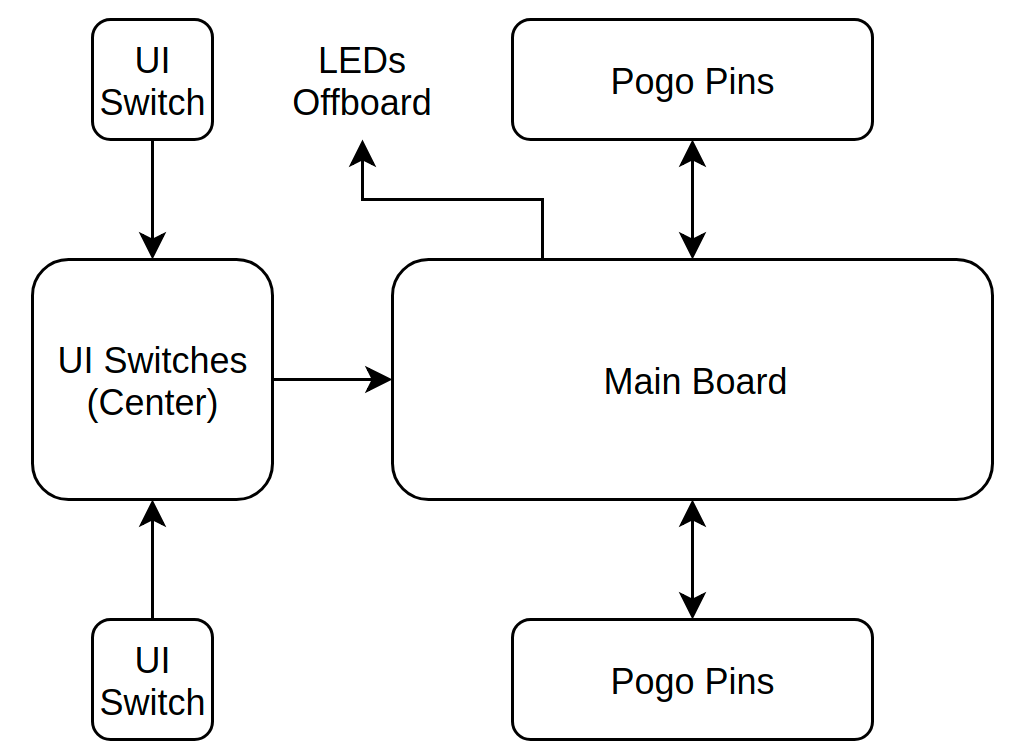
\includegraphics[width = 0.4\textwidth]{PR5Images/PCBHierarchy.png}
		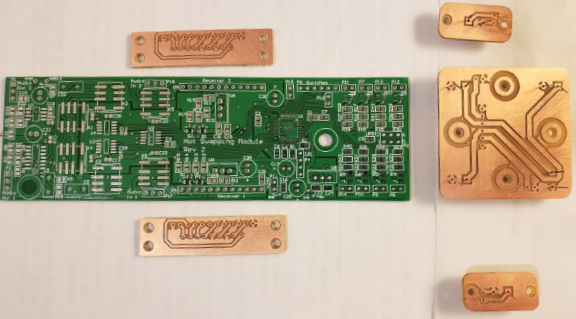
\includegraphics[width = 0.6\textwidth, angle = 180]{PR5Images/PCBs.png}
		\caption{Top: Circuit board hierarchy for each module.  The switch boards are inputs to the main board, the LEDs which are not mounted on any board are outputs, and the hot swapping pogo pins are used for mixed signal communication.  Bottom: image of the physical circuit boards.}
		\label{fig:ModulePCBHierarchy}
	\end{figure}

	Each of the circuit boards is mounted with several 2-56 machine screws, which had a small enough diameter to fit without taking up too much space. The physical constraints for the auxiliary boards were fairly minimal. Large trace widths and spacings were used along with a single sided design to simplify manufacture on the circuit board milling machine. Because so many of these simple boards were needed, it made sense to manufacture them using this method. This also meant that last minute changes could be quickly implemented.

	\subsection{Component Placement and Routing Considerations}

	The main board was designed with more standard fabrication methods in mind because of the relatively fine pitch microcontroller and the complexity of a mixed signal design. The area was divided by signal type into several areas, namely the analog signals of the receivers and signal routing subsystem, the relatively high current digital signals used to drive the relays, the global voltage regulation, and the rest of the digital signals including the microcontroller. Each of these sections was laid out with the aim of reducing noise on the analog signals, in order to maintain the high signal-to-noise ratio required. In particular, each section received its own ground plane, all connected at a single point near the power input to the board. This serves to prevent changes in ground voltage at different locations which could occur during sudden or large current draws. Resistance of the ground trace could result in a V = IR voltage developing. Keeping the ground planes separate helps prevent noise from the digital circuits from being introduced into the analog signal. This division is shown at the bottom of Figure \ref{fig:PCBdivisions}.

	\begin{figure}
		\centering
		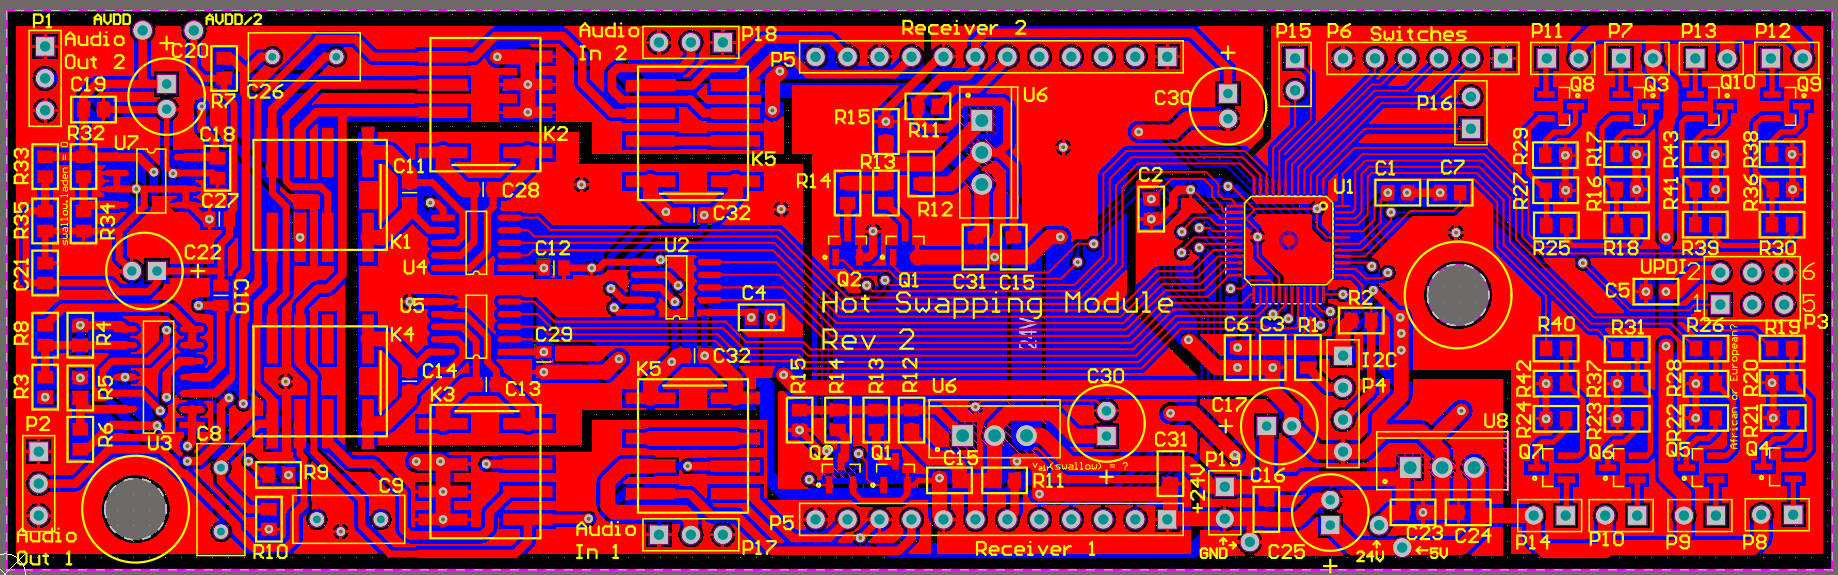
\includegraphics[width = \textwidth]{PR5Images/MainBoard2D.png}
		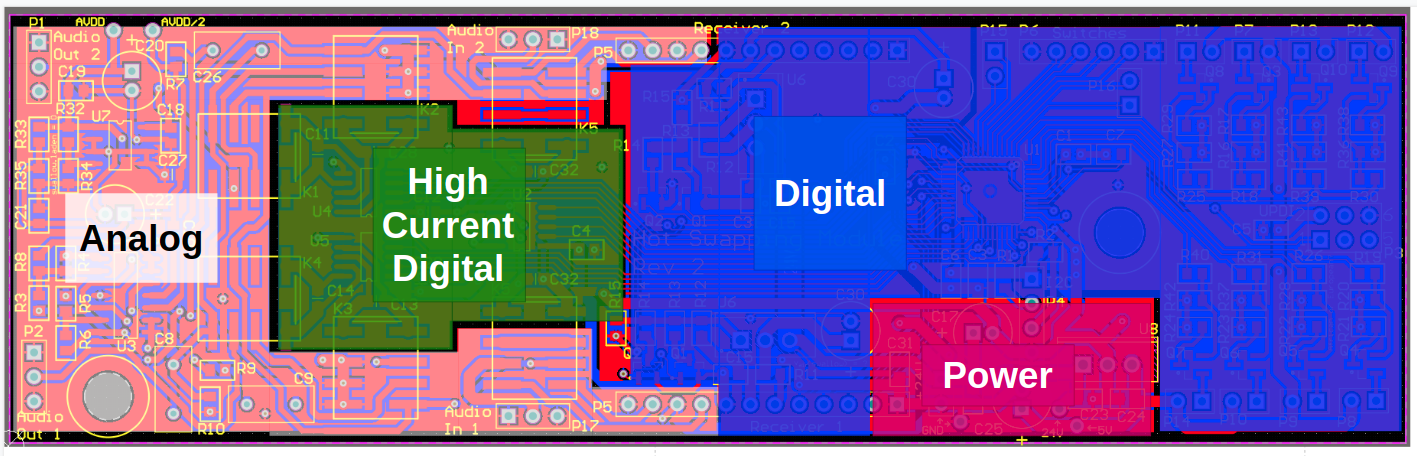
\includegraphics[width = \textwidth]{PR5Images/PCBDivision.png}
		\caption{Top: Main board layout.  Bottom: Ground plane division by signal and function type.}
		\label{fig:PCBdivisions}
	\end{figure}

	To separate the analog digital domains, the components were placed to allow traces of different domains to stay as far away from each other as possible. The relays (K1-5) were oriented so their coils faced onto an inner core while their analog signal connections faced outwards away from the digital control signals. The voltage regulator for the analog summing amplifier was placed close to the amplifier itself to minimize noise from being picked up on a long power trace that would have been necessary if this regulator was placed with the other power supply circuits. The relay drivers were placed as close as possible to their respective relays to minimize the trace resistance on their higher current outputs. This type of optimization helped the device meet the SNR requirement.

\section{Circuit Board Assembly}

	The circuit boards were ordered from a Shenzhen fabrication house under the name JLCPCB, and were received one week after ordering.  The quality of the boards is decent, though one of the cutouts for the standoffs was not cut on any of the boards.  Luckily this is an easily solvable issue, requiring only a drill press.  In addition, the solder mask was misaligned by about 5 mils, which did not prevent assembly in this case but is undesirable; any further would likely not be acceptable.  More troublesome was the procurement of the components, which arrived a few days later than expected, with the thin film audio signal caps backordered.

	Once all of the components arrived, one circuit board was assembled first for verification before the remaining modules were completed, as can be seen in Figure \ref{fig:assembled_pcb}.  The verification of this design indicated that there was only one issue with the design: the wrong footprint was used for the BJTs in the LED constant current drivers.  To fix this, the surface mount transistors were replaced with equivalent through hole devices that were soldered via a number of jumper wires to make the correct connections (this can be seen in the figure).  The rest of the circuit boards including a global I/O board with audio and power connections were fabricated on the milling machine and assembled.  After this first board was verified, three others were assembled, along with their associated peripheral boards.

	\insertimage{0.95}{FinalImages/AssembledPCB.jpg}{Fully assembled main board of module along with global I/O board on top.}{fig:assembled_pcb}

\section{Mechanical Assembly}

	The modular concept that guided the design of this project was combined physically into a single enclosure.  Each subassembly thus far described, including the user interface and receiver systems was designed to mount onto a standardized housing.  In this case, 80-20 1" aluminum extrusion was used to create a rectangular frame 32" x 17".  Each of the subassemblies mounts to this frame using 1/4" machine screws.  The general design is shown in Figure \ref{fig:fullASM}, with the receiver and user interface subassemblies mounted to the frame.  This system of subassemblies allows smaller pieces of material to be used, enabling use of scrap materials for most pieces.  These pieces were cut out of MDF with a CNC router and drill press.

	\begin{figure}
		\centering
		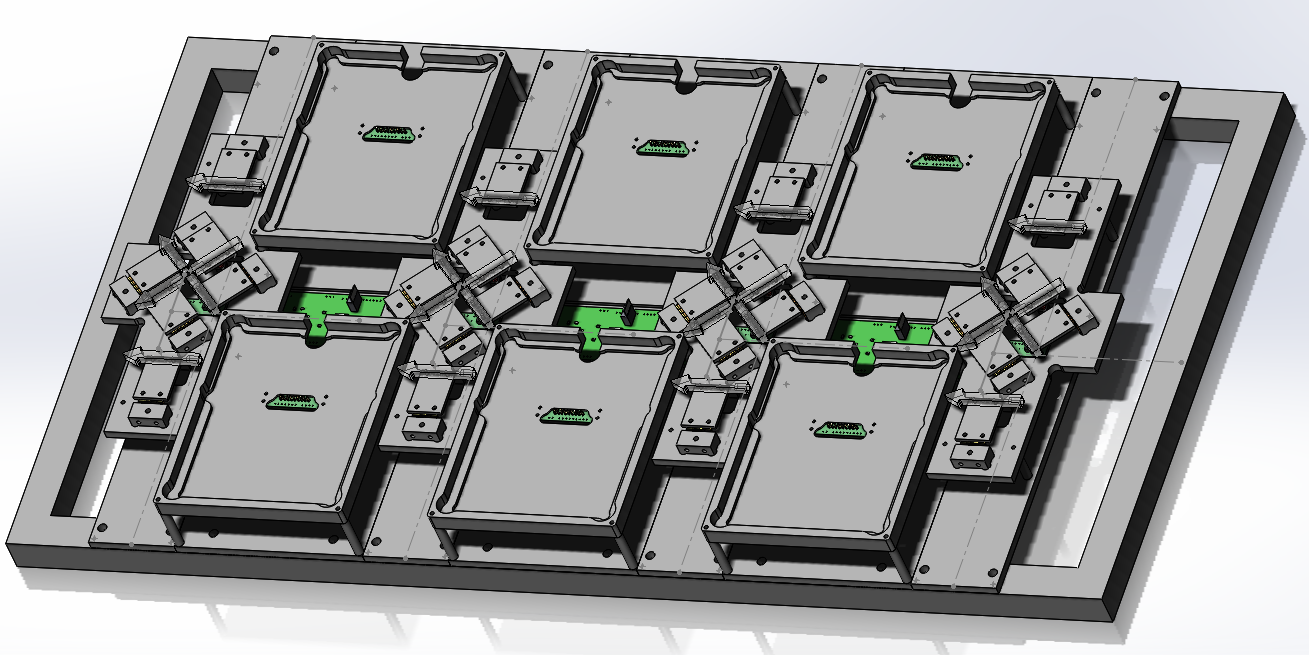
\includegraphics[width = \textwidth]{PR5Images/FullAsmCAD.png}
		\caption{Full scale CAD assembly of device.  The receiver and user interface subassemblies both attach to the frame on the bottom.}
		\label{fig:fullASM}
	\end{figure}

	Because of time constraints, only two sets of modules were integrated into the final constructed design, seen in Figure \ref{fig:fullsystemim}.

	\begin{figure}
		\centering
		\includegraphics[width = \textwidth]{FinalImages/FullSystem}
		\caption{The final product (on a crowded table).  This was used for a live demonstration in the presentation.  Notice the module circuit boards with multi pin cables used to connect peripheral I/O boards to the module, along with global I/O board near the top.}
		\label{fig:fullsystemim}
	\end{figure}


